\documentclass{article}
\usepackage{fullpage}
\usepackage{amsmath}
\usepackage{multicol}
\usepackage{mathptmx}
\usepackage{pgfplots}
\pgfplotsset{compat=1.17}
\usepgfplotslibrary{fillbetween}
\usepackage[aux]{rerunfilecheck}
\usepackage{tikz}
\usetikzlibrary{patterns}

\newcommand{\ds}{\displaystyle}

% Macros for MATH 110 course dates

\newcommand{\commonTheme}{metropolis}
\newcommand{\commonColorTheme}{metropolis}

\newcommand{\commonAuthor}{Edward Doolittle}
\newcommand{\commonInstitute}{Department of Indigenous Knowledge and
  Science \\ First Nations University of Canada}
\newcommand{\commonCourse}{MATH 110 Calculus I}
\newcommand{\commonTerm}{202510}
\newcommand{\commonDate}{January 6, 2025}

% Review Material

% Lab 0
\newcommand{\commonEventNegativeOne}{LabNegativeOne}
\newcommand{\commonDateLabNegativeOne}{Monday, January 6, 2025}
\newcommand{\commonTitleLabNegativeOne}{MATH 110 Lab 0}
\newcommand{\commonSubtitleLabNegativeOne}{No Lab; Course Opens}

% Section 001
\newcommand{\commonEventZeroZeroOne}{ZeroZeroOne}
\newcommand{\commonDateZeroZeroOne}{Tuesday, January 7, 2025}
\newcommand{\commonTitleZeroZeroOne}{MATH 110 Review 0.1}
\newcommand{\commonSubtitleZeroZeroOne}{Review of Algebra}
\newcommand{\commonPSTitleZeroZeroOne}{MATH 110 Review Problem Set 0.1}

% Section 00A
\newcommand{\commonEventZeroZeroA}{ZeroZeroA}
\newcommand{\commonDateZeroZeroA}{Tuesday, January 7, 2025}
\newcommand{\commonTitleZeroZeroA}{MATH 110 Review 0.A}
\newcommand{\commonSubtitleZeroZeroA}{Review of Inequalities and
  Absolute Values}
\newcommand{\commonPSTitleZeroZeroA}{MATH 110 Review Problem Set 0.A}

% Section 00B
\newcommand{\commonEventZeroZeroB}{ZeroZeroB}
\newcommand{\commonDateZeroZeroB}{Tuesday, January 7, 2025}
\newcommand{\commonTitleZeroZeroB}{MATH 110 Review 0.B}
\newcommand{\commonSubtitleZeroZeroB}{Review of Coordinate Geometry
  and Lines}
\newcommand{\commonPSTitleZeroZeroB}{MATH 110 Review Problem Set 0.B}

% Section 00C
\newcommand{\commonEventZeroZeroC}{ZeroZeroC}
\newcommand{\commonDateZeroZeroC}{Thursday, January 9, 2025}
\newcommand{\commonTitleZeroZeroC}{MATH 110 Review 0.C}
\newcommand{\commonSubtitleZeroZeroC}{Review of Graphs of Second
  Degree Equations}
\newcommand{\commonPSTitleZeroZeroC}{MATH 110 Review Problem Set 0.C}

% Section 00D
\newcommand{\commonEventZeroZeroD}{ZeroZeroD}
\newcommand{\commonDateZeroZeroD}{Thursday, January 9, 2025}
\newcommand{\commonTitleZeroZeroD}{MATH 110 Review 0.D}
\newcommand{\commonSubtitleZeroZeroD}{Review of Trigonometry}
\newcommand{\commonPSTitleZeroZeroD}{MATH 110 Review Problem Set 0.D}

% Section 011
\newcommand{\commonEventZeroOneOne}{ZeroOneOne}
\newcommand{\commonDateZeroOneOne}{Thursday, January 9, 2025}
\newcommand{\commonTitleZeroOneOne}{MATH 110 Review 1.1}
\newcommand{\commonSubtitleZeroOneOne}{Review of Functions}
\newcommand{\commonPSTitleZeroOneOne}{MATH 110 Review Problem Set 1.1}


% Main Course

% Lab 1
\newcommand{\commonEventZero}{LabZero}
\newcommand{\commonDateLabZero}{Monday, January 13, 2025}
\newcommand{\commonTitleLabZero}{MATH 110 Lab 1}
\newcommand{\commonSubtitleLabZero}{Quiz 0: STACK, Onboarding}

% Section 1.4
\newcommand{\commonEventOne}{ZeroOneFour}
\newcommand{\commonDateZeroOneFour}{Tuesday, January 14, 2025}
\newcommand{\commonTitleZeroOneFour}{MATH 110 Lecture 1.4}
\newcommand{\commonSubtitleZeroOneFour}{The Tangent and Velocity Problems}
\newcommand{\commonPSTitleZeroOneFour}{MATH 110 Problem Set 1.4}

% Section 1.5
\newcommand{\commonEventTwo}{ZeroOneFive}
\newcommand{\commonDateZeroOneFive}{Thursday, January 16, 2025}
\newcommand{\commonTitleZeroOneFive}{MATH 110 Lecture 1.5}
\newcommand{\commonSubtitleZeroOneFive}{The Limit of a Function}
\newcommand{\commonPSTitleZeroOneFive}{MATH 110 Problem Set 1.5}

% Lab 2
\newcommand{\commonEventThree}{LabOne}
\newcommand{\commonDateLabOne}{Monday, January 20, 2025}
\newcommand{\commonTitleLabOne}{MATH 110 Lab 2}
\newcommand{\commonSubtitleLabOne}{Quiz 1: Review}

% Section 1.6
\newcommand{\commonEventFour}{ZeroOneSix}
\newcommand{\commonDateZeroOneSix}{Tuesday, January 21, 2025}
\newcommand{\commonTitleZeroOneSix}{MATH 110 Lecture 1.6}
\newcommand{\commonSubtitleZeroOneSix}{Calculating Limits Using the Limit Laws}
\newcommand{\commonPSTitleZeroOneSix}{MATH 110 Problem Set 1.6}

% Section 1.7
\newcommand{\commonEventFive}{ZeroOneSeven}
\newcommand{\commonDateZeroOneSeven}{(Not covered)}
\newcommand{\commonTitleZeroOneSeven}{MATH 110 Lecture 1.7}
\newcommand{\commonSubtitleZeroOneSeven}{The Precise Definition of a Limit}
\newcommand{\commonPSTitleZeroOneSeven}{MATH 110 Problem Set 1.7}

% Section 1.8
\newcommand{\commonEventSix}{ZeroOneEight}
\newcommand{\commonDateZeroOneEight}{Thursday, January 23, 2025}
\newcommand{\commonTitleZeroOneEight}{MATH 110 Lecture 1.8}
\newcommand{\commonSubtitleZeroOneEight}{Continuity}
\newcommand{\commonPSTitleZeroOneEight}{MATH 110 Problem Set 1.8}

% Lab 3
\newcommand{\commonEventSeven}{LabTwo}
\newcommand{\commonDateLabTwo}{Monday, January 27, 2025}
\newcommand{\commonTitleLabTwo}{MATH 110 Lab 3}
\newcommand{\commonSubtitleLabTwo}{Quiz 2: Sections 1.4, 1.5}

% Section 2.1
\newcommand{\commonEventEight}{ZeroTwoOne}
\newcommand{\commonDateZeroTwoOne}{Tuesday, January 28, 2025}
\newcommand{\commonTitleZeroTwoOne}{MATH 110 Lecture 2.1}
\newcommand{\commonSubtitleZeroTwoOne}{Derivatives and Rates of Change}
\newcommand{\commonPSTitleZeroTwoOne}{MATH 110 Problem Set 2.1}

% Section 2.2
\newcommand{\commonEventNine}{ZeroTwoTwo}
\newcommand{\commonDateZeroTwoTwo}{Thursday, January 30, 2025}
\newcommand{\commonTitleZeroTwoTwo}{MATH 110 Lecture 2.2}
\newcommand{\commonSubtitleZeroTwoTwo}{The Derivative as a Function}
\newcommand{\commonPSTitleZeroTwoTwo}{MATH 110 Problem Set 2.2}

% Lab 4
\newcommand{\commonEventTen}{LabThree}
\newcommand{\commonDateMTOne}{Monday, February 3, 2025} 
\newcommand{\commonDateLabThree}{Monday, February 3, 2025}
\newcommand{\commonTitleLabThree}{MATH 110 Lab 4}
\newcommand{\commonSubtitleLabThree}{Midterm: Review, Chapter 1}

% Section 2.3
\newcommand{\commonEventEleven}{ZeroTwoThree}
\newcommand{\commonDateZeroTwoThree}{Tuesday, February 4, 2025}
\newcommand{\commonTitleZeroTwoThree}{MATH 110 Lecture 2.3}
\newcommand{\commonSubtitleZeroTwoThree}{Differentiation Formulas}
\newcommand{\commonPSTitleZeroTwoThree}{MATH 110 Problem Set 2.3}

% Section 2.4
\newcommand{\commonEventTwelve}{ZeroTwoFour}
\newcommand{\commonDateZeroTwoFour}{Thursday, February 6, 2025}
\newcommand{\commonTitleZeroTwoFour}{MATH 110 Lecture 2.4}
\newcommand{\commonSubtitleZeroTwoFour}{Derivatives of Trigonometric Functions}
\newcommand{\commonPSTitleZeroTwoFour}{MATH 110 Problem Set 2.4}

% Lab 5
\newcommand{\commonEventThirteen}{LabFour}
\newcommand{\commonDateLabFour}{Monday, February 10, 2025}
\newcommand{\commonTitleLabFour}{MATH 110 Lab 5}
\newcommand{\commonSubtitleLabFour}{Quiz 3: Sections 2.1, 2.2}

% Section 2.5
\newcommand{\commonEventFourteen}{ZeroTwoFive}
\newcommand{\commonDateZeroTwoFive}{Tuesday, February 11, 2025}
\newcommand{\commonTitleZeroTwoFive}{MATH 110 Lecture 2.5}
\newcommand{\commonSubtitleZeroTwoFive}{The Chain Rule}
\newcommand{\commonPSTitleZeroTwoFive}{MATH 110 Problem Set 2.5}

% Section 2.6
\newcommand{\commonEventFifteen}{ZeroTwoSix}
\newcommand{\commonDateZeroTwoSix}{Thursday, February 13, 2025}
\newcommand{\commonTitleZeroTwoSix}{MATH 110 Lecture 2.6}
\newcommand{\commonSubtitleZeroTwoSix}{Implicit Differentiation}
\newcommand{\commonPSTitleZeroTwoSix}{MATH 110 Problem Set 2.6}

% Lab 6
\newcommand{\commonEventSixteen}{LabFive}
\newcommand{\commonDateLabFive}{Monday, February 24, 2025}
\newcommand{\commonTitleLabFive}{MATH 110 Lab 6}
\newcommand{\commonSubtitleLabFive}{Quiz 4: Sections 2.3, 2.4}

% Section 2.7
\newcommand{\commonEventSeventeen}{ZeroTwoSeven}
\newcommand{\commonDateZeroTwoSeven}{Tuesday, February 25, 2025}
\newcommand{\commonTitleZeroTwoSeven}{MATH 110 Lecture 2.7}
\newcommand{\commonSubtitleZeroTwoSeven}{Rates of Change in the
  Natural and Social Sciences}
\newcommand{\commonPSTitleZeroTwoSeven}{MATH 110 Problem Set 2.7}

% Section 2.8
\newcommand{\commonEventEighteen}{ZeroTwoEight}
\newcommand{\commonDateZeroTwoEight}{Thursday, February 27, 2025}
\newcommand{\commonTitleZeroTwoEight}{MATH 110 Lecture 2.8}
\newcommand{\commonSubtitleZeroTwoEight}{Related Rates}
\newcommand{\commonPSTitleZeroTwoEight}{MATH 110 Problem Set 2.8}

% Lab 7
\newcommand{\commonEventNineteen}{LabSix}
\newcommand{\commonDateLabSix}{Monday, March 3, 2025}
\newcommand{\commonTitleLabSix}{MATH 110 Lab 7}
\newcommand{\commonSubtitleLabSix}{Quiz 5: Sections 2.5, 2.6}

% Section 3.1
\newcommand{\commonEventTwenty}{ZeroThreeOne}
\newcommand{\commonDateZeroThreeOne}{Tuesday, March 4, 2025}
\newcommand{\commonTitleZeroThreeOne}{MATH 110 Lecture 3.1}
\newcommand{\commonSubtitleZeroThreeOne}{Maximum and Minimum Values}
\newcommand{\commonPSTitleZeroThreeOne}{MATH 11 Problem Set 3.1}

% Section 3.2
\newcommand{\commonEventTwentyOne}{ZeroThreeTwo}
\newcommand{\commonDateZeroThreeTwo}{Thursday, March 6, 2025}
\newcommand{\commonTitleZeroThreeTwo}{MATH 110 Lecture 3.2}
\newcommand{\commonSubtitleZeroThreeTwo}{The Mean Value Theorem}
\newcommand{\commonPSTitleZeroThreeTwo}{MATH 110 Problem Set 3.2}

% Lab 8
\newcommand{\commonEventTwentyTwo}{LabSeven}
\newcommand{\commonDateMTTwo}{Monday, March 10, 2025}
\newcommand{\commonDateLabSeven}{Monday, March 10, 2025}
\newcommand{\commonTitleLabSeven}{MATH 110 Lab 8}
\newcommand{\commonSubtitleLabSeven}{Midterm: Chapter 2}

% Section 3.3
\newcommand{\commonEventTwentyThree}{ZeroThreeThree}
\newcommand{\commonDateZeroThreeThree}{Tuesday, March 11, 2025}
\newcommand{\commonTitleZeroThreeThree}{MATH 110 Lecture 3.3}
\newcommand{\commonSubtitleZeroThreeThree}{How Derivatives Affect the
  Shape of a Graph}
\newcommand{\commonPSTitleZeroThreeThree}{MATH 110 Problem Set 3.3}

% Section 3.4
\newcommand{\commonEventTwentyFour}{ZeroThreeFour}
\newcommand{\commonDateZeroThreeFour}{Thursday, March 13, 2025}
\newcommand{\commonTitleZeroThreeFour}{MATH 110 Lecture 3.4}
\newcommand{\commonSubtitleZeroThreeFour}{Limits at Infinity;
  Horizontal Asymptotes}
\newcommand{\commonPSTitleZeroThreeFour}{MATH 110 Problem Set 3.4}

% Lab 9
\newcommand{\commonEventTwentyFive}{LabEight}
\newcommand{\commonDateLabEight}{Monday, March 17, 2025}
\newcommand{\commonTitleLabEight}{MATH 110 Lab 9}
\newcommand{\commonSubtitleLabEight}{Quiz 6: Sections 3.1, 3.2}

% Section 3.5
\newcommand{\commonEventTwentySix}{ZeroThreeFive}
\newcommand{\commonDateZeroThreeFive}{Tuesday, March 18, 2025}
\newcommand{\commonTitleZeroThreeFive}{MATH 110 Lecture 3.5}
\newcommand{\commonSubtitleZeroThreeFive}{Summary of Curve Sketching}
\newcommand{\commonPSTitleZeroThreeFive}{MATH 110 Problem Set 3.5}

% Section 3.7
\newcommand{\commonEventTwentySeven}{ZeroThreeSeven}
\newcommand{\commonDateZeroThreeSeven}{Thursday, March 20, 2025}
\newcommand{\commonTitleZeroThreeSeven}{MATH 110 Lecture 3.7}
\newcommand{\commonSubtitleZeroThreeSeven}{Optimization Problems}
\newcommand{\commonPSTitleZeroThreeSeven}{MATH 110 Problem Set 3.7}

% Lab 10
\newcommand{\commonEventTwentyEight}{LabNine}
\newcommand{\commonDateLabNine}{Monday, March 24, 2025}
\newcommand{\commonTitleLabNine}{MATH 110 Lab 10}
\newcommand{\commonSubtitleLabNine}{Quiz 7: Sections 3.3, 3.4}

% Section 4.1
\newcommand{\commonEventTwentyNine}{ZeroFourOne}
\newcommand{\commonDateZeroFourOne}{Tuesday, March 25, 2025}
\newcommand{\commonTitleZeroFourOne}{MATH 110 Lecture 4.1}
\newcommand{\commonSubtitleZeroFourOne}{Areas and Distances}
\newcommand{\commonPSTitleZeroFourOne}{MATH 110 Problem Set 4.1}

% Section 4.2
\newcommand{\commonEventThirty}{ZeroFourTwo}
\newcommand{\commonDateZeroFourTwo}{Thursday, March 27, 2025}
\newcommand{\commonTitleZeroFourTwo}{MATH 110 Lecture 4.2}
\newcommand{\commonSubtitleZeroFourTwo}{The Definite Integral}
\newcommand{\commonPSTitleZeroFourTwo}{MATH 110 Problem Set 4.2}

% Lab 11
\newcommand{\commonEventThirtyOne}{LabTen}
\newcommand{\commonDateLabTen}{Monday, March 31, 2025}
\newcommand{\commonTitleLabTen}{MATH 110 Lab 11}
\newcommand{\commonSubtitleLabTen}{Quiz 8: Sections 3.5, 3.7}

% Section 4.3
\newcommand{\commonEventThirtyTwo}{ZeroFourThree}
\newcommand{\commonDateZeroFourThree}{Tuesday, April 1, 2025}
\newcommand{\commonTitleZeroFourThree}{MATH 110 Lecture 4.3}
\newcommand{\commonSubtitleZeroFourThree}{The Fundamental Theorem of Calculus}
\newcommand{\commonPSTitleZeroFourThree}{MATH 110 Problem Set 4.3}

% Section 4.4
\newcommand{\commonEventThirtyThree}{ZeroFourFour}
\newcommand{\commonDateZeroFourFour}{Thursday, April 3, 2025}
\newcommand{\commonTitleZeroFourFour}{MATH 110 Lecture 4.4}
\newcommand{\commonSubtitleZeroFourFour}{Indefinite Integrals and the
  Net Change Theorem}
\newcommand{\commonPSTitleZeroFourFour}{MATH 110 Problem Set 4.4}

% Lab 12
\newcommand{\commonEventThirtyFour}{LabEleven}
\newcommand{\commonDateLabEleven}{Monday, April 7, 2025}
\newcommand{\commonTitleLabEleven}{MATH 110 Lab 12}
\newcommand{\commonSubtitleLabEleven}{Quiz 9: Sections 4.1, 4.2}

% Section 4.5
\newcommand{\commonEventThirtyFive}{ZeroFourFive}
\newcommand{\commonDateZeroFourFive}{Tuesday, April 8, 2025}
\newcommand{\commonTitleZeroFourFive}{MATH 110 Lecture 4.5}
\newcommand{\commonSubtitleZeroFourFive}{The Substitution Rule}
\newcommand{\commonPSTitleZeroFourFive}{MATH 110 Problem Set 4.5}

% Section 5.1
\newcommand{\commonEventThirtySix}{ZeroFiveOne}
\newcommand{\commonDateZeroFiveOne}{Thursday, April 10, 2025}
\newcommand{\commonTitleZeroFiveOne}{MATH 110 Lecture 5.1}
\newcommand{\commonSubtitleZeroFiveOne}{Areas Between Curves}
\newcommand{\commonPSTitleZeroFiveOne}{MATH 110 Problem Set 5.1}

% Lab 13
\newcommand{\commonEventThirtySeven}{LabTwelve}
\newcommand{\commonDateLabTwelve}{Monday, April 14, 2025}
\newcommand{\commonTitleLabTwelve}{MATH 110 Review Lab}
\newcommand{\commonSubtitleLabTwelve}{Bonus Quiz 10: Sections 4.3, 4.4}

% Final Class
\newcommand{\commonEventThirtyEight}{FinalClass}
\newcommand{\commonDateFinalClass}{Tuesday, April 15, 2025}
\newcommand{\commonTitleFinalClass}{MATH 110 Review Class}
\newcommand{\commonSubtitleFinalClass}{Answer Questions, Review for Exam}

% Final Exam
\newcommand{\commonEventThirtyNine}{Final}
\newcommand{\commonDateFinal}{Thursday, April 22, 2025}
\newcommand{\commonTitleFinal}{MATH 110 Final Exam}
\newcommand{\commonSubtitleFinal}{Comprehensive Exam: All Sections}

% Orphaned -- no longer part of the course

% Section 2.9
\newcommand{\commonDateZeroTwoNine}{Not part of the course}
\newcommand{\commonTitleZeroTwoNine}{MATH 110 Lecture 2.9}
\newcommand{\commonSubtitleZeroTwoNine}{Linear Approximations and Differentials}
\newcommand{\commonPSTitleZeroTwoNine}{MATH 110 Problem Set 2.9}


% % Introduction
% \newcommand{\commonEventOneDate}{Wednesday, September 8, 2010}
% \newcommand{\commonEventOneDesc}{Introduction to the Course}
% \newcommand{\commonDateZeroZeroZero}{September 8, 2010}
% \newcommand{\commonTitleZeroZeroZero}{MATH 104 Introduction}
% \newcommand{\commonSubtitleZeroZeroZero}{Outline of the Course}

% % Lecture 1
% \newcommand{\commonEventTwoDate}{Friday, September 10, 2010}
% \newcommand{\commonEventTwoDesc}{Lecture 1: Algebra}
% \newcommand{\commonDateZeroZeroOne}{September 10, 2010}
% \newcommand{\commonTitleZeroZeroOne}{MATH 104 Lecture 1}
% \newcommand{\commonSubtitleZeroZeroOne}{Review of Algebra}
% % associated evaluation ... factor this out?
% \newcommand{\commonPSTitleZeroZeroOne}{MATH 104 Problem Set 1}
% \newcommand{\commonEvalZeroZeroOne}{Quiz 1}
% \newcommand{\commonEvalDateZeroZeroOne}{Wednesday, September 15, 2010}

% % Lecture 2
% \newcommand{\commonEventThreeDate}{Monday, September 13, 2010}
% \newcommand{\commonEventThreeDesc}{Lecture 2: Appendix A}
% \newcommand{\commonDateZeroZeroA}{September 13, 2010}
% \newcommand{\commonTitleZeroZeroA}{MATH 104 Lecture 2}
% \newcommand{\commonSubtitleZeroZeroA}{Appendix A: Numbers, Inequalities, 
%   and Absolute Values}
% % associated evaluation ... factor this out?
% \newcommand{\commonPSTitleZeroZeroA}{MATH 104 Problem Set 2}
% \newcommand{\commonEvalZeroZeroA}{Quiz 2}
% \newcommand{\commonEvalDateZeroZeroA}{Wednesday, September 22, 2010}

% % Review 1
% \newcommand{\commonEventFourDate}{Wednesday, September 15, 2010}
% \newcommand{\commonEventFourDesc}{Review 1: Review Algebra; Quiz 1; Review Appendix A}
% \newcommand{\commonDateRZeroOne}{September 15, 2010}
% \newcommand{\commonTitleRZeroOne}{MATH 104 Review 1}
% \newcommand{\commonSubtitleRZeroOne}{Review of Algebra, Appendix A}

% % Lecture 3
% \newcommand{\commonEventFiveDate}{Friday, September 17, 2010}
% \newcommand{\commonEventFiveDesc}{Lecture 3: Appendix B}
% \newcommand{\commonDateZeroZeroB}{September 17, 2010}
% \newcommand{\commonTitleZeroZeroB}{MATH 104 Lecture 3}
% \newcommand{\commonSubtitleZeroZeroB}{Appendix B: Coordinate Geometry and Lines}
% % associated evaluation ... factor this out?
% \newcommand{\commonPSTitleZeroZeroB}{MATH 104 Problem Set 3}
% \newcommand{\commonEvalZeroZeroB}{Quiz 2}
% \newcommand{\commonEvalDateZeroZeroB}{Wednesday, September 22, 2010}

% % Lecture 4
% \newcommand{\commonEventSixDate}{Monday, Sepbember 20, 2010}
% \newcommand{\commonEventSixDesc}{Lecture 4: Appendix C}
% \newcommand{\commonDateZeroZeroC}{September 20, 2010}
% \newcommand{\commonTitleZeroZeroC}{MATH 104 Lecture 4}
% \newcommand{\commonSubtitleZeroZeroC}{Appendix C: Graphs of Second-Degree Equations}
% % associated evaluation ... factor this out?
% \newcommand{\commonPSTitleZeroZeroC}{MATH 104 Problem Set 4}
% \newcommand{\commonEvalZeroZeroC}{Midterm 0}
% \newcommand{\commonEvalDateZeroZeroC}{Wednesday, September 29, 2010}

% % Review 2
% \newcommand{\commonEventSevenDate}{Wednesday, September 22, 2010}
% \newcommand{\commonEventSevenDesc}{Review 2: Review Appendix B; Quiz 2; Review Appendix C}
% \newcommand{\commonDateRZeroTwo}{September 22, 2010}
% \newcommand{\commonTitleRZeroTwo}{MATH 104 Review 2}
% \newcommand{\commonSubtitleRZeroTwo}{Review of Appendices B and C}

% % Lecture 5
% \newcommand{\commonEventEightDate}{Friday, September 24, 2010}
% \newcommand{\commonEventEightDesc}{Lecture 5: Appendix D}
% \newcommand{\commonDateZeroZeroD}{September 24, 2010}
% \newcommand{\commonTitleZeroZeroD}{MATH 104 Lecture 5}
% \newcommand{\commonSubtitleZeroZeroD}{Appendix D: Trigonometry}
% % associated evaluation ... factor this out?
% \newcommand{\commonPSTitleZeroZeroD}{MATH 104 Problem Set 5}
% \newcommand{\commonEvalZeroZeroD}{Midterm 0}
% \newcommand{\commonEvalDateZeroZeroD}{Wednesday, September 29, 2010}

% % Lecture 6
% \newcommand{\commonEventNineDate}{Monday, September 27, 2010}
% \newcommand{\commonEventNineDesc}{Lecture 6: Section 1.1}
% \newcommand{\commonDateZeroOneOne}{September 27, 2010}
% \newcommand{\commonTitleZeroOneOne}{MATH 104 Lecture 6}
% \newcommand{\commonSubtitleZeroOneOne}{Section 1.1: Four Ways to Represent a Function}
% % associated evaluation ... factor this out?
% \newcommand{\commonPSTitleZeroOneOne}{MATH 104 Problem Set 6}
% \newcommand{\commonEvalZeroOneOne}{Quiz 3}
% \newcommand{\commonEvalDateZeroOneOne}{Wednesday, October 6, 2010}

% % Review 3
% \newcommand{\commonEventTenDate}{Wednesday, September 29, 2010}
% \newcommand{\commonEventTenDesc}{Review 3: Review Appendix D; 
%   Self-Assessment Midterm 0}
% \newcommand{\commonDateRZeroThree}{September 29, 2010}
% \newcommand{\commonTitleRZeroThree}{MATH 104 Review 3}
% \newcommand{\commonSubtitleRZeroThree}{Review of Appendix D}

% % Lecture 7
% \newcommand{\commonEventElevenDate}{Friday, October 1, 2010}
% \newcommand{\commonEventElevenDesc}{Lecture 7: Section 1.2}
% \newcommand{\commonDateZeroOneTwo}{October 1, 2010}
% \newcommand{\commonTitleZeroOneTwo}{MATH 104 Lecture 7}
% \newcommand{\commonSubtitleZeroOneTwo}{Section 1.2: Mathematical Models: A Catalog of Essential Functions}
% % associated evaluation ... factor this out?
% \newcommand{\commonPSTitleZeroOneTwo}{MATH 104 Problem Set 7}
% \newcommand{\commonEvalZeroOneTwo}{Quiz 3}
% \newcommand{\commonEvalDateZeroOneTwo}{Wednesday, October 6, 2010}

% % Lecture 8
% \newcommand{\commonEventTwelveDate}{Monday, October 4, 2010}
% \newcommand{\commonEventTwelveDesc}{Lecture 8: Section 1.3}
% \newcommand{\commonDateZeroOneThree}{October 4, 2010}
% \newcommand{\commonTitleZeroOneThree}{MATH 104 Lecture 8}
% \newcommand{\commonSubtitleZeroOneThree}{Section 1.3: New Functions from Old Functions}
% % associated evaluation ... factor this out?
% \newcommand{\commonPSTitleZeroOneThree}{MATH 104 Problem Set 8}
% \newcommand{\commonEvalZeroOneThree}{Quiz 4}
% \newcommand{\commonEvalDateZeroOneThree}{Wednesday, October 13, 2010}

% % Review 4
% \newcommand{\commonEventThirteenDate}{Wednesday, October 6, 2010}
% \newcommand{\commonEventThirteenDesc}{Review 4: Review 1.1, 1.2; Quiz 3}
% \newcommand{\commonDateROneOne}{October 6, 2010}
% \newcommand{\commonTitleROneOne}{MATH 104 Review 4}
% \newcommand{\commonSubtitleROneOne}{Reveiw of 1.1, 1.2}

% % Lecture 9
% \newcommand{\commonEventFourteenDate}{Friday, October 8, 2010}
% \newcommand{\commonEventFourteenDesc}{Lecture 9: Section 1.4}
% \newcommand{\commonDateZeroOneFour}{October 8, 2010}
% \newcommand{\commonTitleZeroOneFour}{MATH 104 Lecture 9}
% \newcommand{\commonSubtitleZeroOneFour}{Section 1.4: Graphing Calculators and Computers}
% % associated evaluation ... factor this out?
% \newcommand{\commonPSTitleZeroOneFour}{MATH 104 Problem Set 9}
% \newcommand{\commonEvalZeroOneFour}{Quiz 4}
% \newcommand{\commonEvalDateZeroOneFour}{Wednesday, October 13, 2010}

% % Thanksgiving holiday
% \newcommand{\commonEventFifteenDate}{Monday, October 11, 2010}
% \newcommand{\commonEventFifteenDesc}{No class: Thanksgiving holiday}

% % Review 5
% \newcommand{\commonEventSixteenDate}{Wednesday, October 13, 2010}
% \newcommand{\commonEventSixteenDesc}{Review 5: Review 1.3, 1.4; Quiz 4}
% \newcommand{\commonDateROneTwo}{October 13, 2010}
% \newcommand{\commonTitleROneTwo}{MATH 104 Review 5}
% \newcommand{\commonSubtitleOneRTwo}{Review of 1.3, 1.4}

% % Lecture 10
% \newcommand{\commonEventSeventeenDate}{Friday, October 15, 2010}
% \newcommand{\commonEventSeventeenDesc}{Lecture 10: Section 1.5}
% \newcommand{\commonDateZeroOneFive}{October 15, 2010}
% \newcommand{\commonTitleZeroOneFive}{MATH 104 Lecture 10}
% \newcommand{\commonSubtitleZeroOneFive}{Section 1.5: Exponential Functions}
% % associated evaluation ... factor this out?
% \newcommand{\commonPSTitleZeroOneFive}{MATH 104 Problem Set 10}
% \newcommand{\commonEvalZeroOneFive}{Quiz 5}
% \newcommand{\commonEvalDateZeroOneFive}{Wednesday, October 20, 2010}

% % Lecture 11
% \newcommand{\commonEventEighteenDate}{Monday, October 18, 2010}
% \newcommand{\commonEventEighteenDesc}{Lecture 11: Section 1.6}
% \newcommand{\commonDateZeroOneSix}{October 18, 2010}
% \newcommand{\commonTitleZeroOneSix}{MATH 104 Lecture 11}
% \newcommand{\commonSubtitleZeroOneSix}{Section 1.6: Inverse Functions and Logarithms}
% % associated evaluation ... factor this out?
% \newcommand{\commonPSTitleZeroOneSix}{MATH 104 Problem Set 11}
% \newcommand{\commonEvalZeroOneSix}{Midterm 1}
% \newcommand{\commonEvalDateZeroOneSix}{Wednesday, October 27, 2010}

% % Review 6
% \newcommand{\commonEventNineteenDate}{Wednesday, October 20, 2010}
% \newcommand{\commonEventNineteenDesc}{Review 6: Review 1.5; Quiz 5; Review 1.6}
% \newcommand{\commonDateROneThree}{October 20, 2010}
% \newcommand{\commonDateZeroOneR}{October 20, 2010}
% \newcommand{\commonTitleROneThree}{MATH 104 Review 6}
% \newcommand{\commonSubtitleROneThree}{Review of 1.5, 1.6}
% % associated evaluation ... factor this out?
% \newcommand{\commonPSTitleZeroOneR}{MATH 104 Problem Set R1}
% \newcommand{\commonEvalZeroOneR}{Midterm 1}
% \newcommand{\commonEvalDateZeroOneR}{Wednesday, October 27, 2010}

% % Lecture 12
% \newcommand{\commonEventTwentyDate}{Friday, October 22, 2010}
% \newcommand{\commonEventTwentyDesc}{Lecture 12: Section 2.1}
% \newcommand{\commonDateZeroTwoOne}{October 22, 2010}
% \newcommand{\commonTitleZeroTwoOne}{MATH 104 Lecture 12}
% \newcommand{\commonSubtitleZeroTwoOne}{Section 2.1: The Tangent and Velocity Problems}
% % associated evaluation ... factor this out?
% \newcommand{\commonPSTitleZeroTwoOne}{MATH 104 Problem Set 12}
% \newcommand{\commonEvalZeroTwoOne}{Quiz 6}
% \newcommand{\commonEvalDateZeroTwoOne}{Wednesday, November 3, 2010}

% % Lecture 13
% \newcommand{\commonEventTwentyOneDate}{Monday, October 25, 2010}
% \newcommand{\commonEventTwentyOneDesc}{Lecture 13: Section 2.2(a)}
% \newcommand{\commonDateZeroTwoTwoa}{October 25, 2010}
% \newcommand{\commonTitleZeroTwoTwoa}{MATH 104 Lecture 13}
% \newcommand{\commonSubtitleZeroTwoTwoa}{Section 2.2(a): The Limit of a Function I}
% % associated evaluation ... factor this out?
% \newcommand{\commonPSTitleZeroTwoTwoa}{MATH 104 Problem Set 13}
% \newcommand{\commonEvalZeroTwoTwoa}{Quiz 6}
% \newcommand{\commonEvalDateZeroTwoTwoa}{Wednesday, November 3, 2010}

% % Midterm Test 1
% % October 27, 2010
% \newcommand{\commonEventTwentyTwoDate}{Wednesday, October 27, 2010}
% \newcommand{\commonEventTwentyTwoDesc}{Midterm Test 1: Chapter 1}

% % Lecture 14
% \newcommand{\commonEventTwentyThreeDate}{Friday, October 29, 2010}
% \newcommand{\commonEventTwentyThreeDesc}{Lecture 14: Section 2.2(b)}
% \newcommand{\commonDateZeroTwoTwob}{October 29, 2010}
% \newcommand{\commonTitleZeroTwoTwob}{MATH 104 Lecture 14}
% \newcommand{\commonSubtitleZeroTwoTwob}{Section 2.2(b): The Limit of a Function II}
% % associated evaluation ... factor this out?
% \newcommand{\commonPSTitleZeroTwoTwob}{MATH 104 Problem Set 14}
% \newcommand{\commonEvalZeroTwoTwob}{Quiz 6}
% \newcommand{\commonEvalDateZeroTwoTwob}{Wednesday, November 3, 2010}

% % Lecture 15
% \newcommand{\commonEventTwentyFourDate}{Monday, November 1, 2010}
% \newcommand{\commonEventTwentyFourDesc}{Lecture 15: Section 2.3}
% \newcommand{\commonDateZeroTwoThree}{November 1, 2010}
% \newcommand{\commonTitleZeroTwoThree}{MATH 104 Lecture 15}
% \newcommand{\commonSubtitleZeroTwoThree}{Section 2.3: Calculating Limits Using the Limit Laws}
% % associated evaluation ... factor this out?
% \newcommand{\commonPSTitleZeroTwoThree}{MATH 104 Problem Set 15}
% \newcommand{\commonEvalZeroTwoThree}{Quiz 7}
% \newcommand{\commonEvalDateZeroTwoThree}{Wednesday, November 10, 2010}

% % Review 7
% \newcommand{\commonEventTwentyFiveDate}{Wednesday, November 3, 2010}
% \newcommand{\commonEventTwentyFiveDesc}{Review 7: Review 2.1, 2.2; Quiz 6; Review 2.3}
% \newcommand{\commonDateRTwoOne}{November 3, 2010}
% \newcommand{\commonTitleRTwoOne}{MATH 104 Review 7}
% \newcommand{\commonSubtitleRTwoOne}{Review of 2.1, 2.2, 2.3}

% % Lecture 16
% \newcommand{\commonEventTwentySixDate}{Friday, November 5, 2010}
% \newcommand{\commonEventTwentySixDesc}{Lecture 16: Section 2.5}
% \newcommand{\commonDateZeroTwoFive}{November 5, 2010}
% \newcommand{\commonTitleZeroTwoFive}{MATH 104 Lecture 16}
% \newcommand{\commonSubtitleZeroTwoFive}{Section 2.5: Continuity}
% % associated evaluation ... factor this out?
% \newcommand{\commonPSTitleZeroTwoFive}{MATH 104 Problem Set 16}
% \newcommand{\commonEvalZeroTwoFive}{Quiz 7}
% \newcommand{\commonEvalDateZeroTwoFive}{Wednesday, November 10, 2010}

% % Lecture 17
% \newcommand{\commonEventTwentySevenDate}{Monday, November 8, 2010}
% \newcommand{\commonEventTwentySevenDesc}{Lecture 17: Section 2.6}
% \newcommand{\commonDateZeroTwoSix}{November 8, 2010}
% \newcommand{\commonTitleZeroTwoSix}{MATH 104 Lecture 17}
% \newcommand{\commonSubtitleZeroTwoSix}{Section 2.6: Limits at Infinity: Horizontal Asymptotes}
% % associated evaluation ... factor this out?
% \newcommand{\commonPSTitleZeroTwoSix}{MATH 104 Problem Set 17}
% \newcommand{\commonEvalZeroTwoSix}{Quiz 8}
% \newcommand{\commonEvalDateZeroTwoSix}{Wednesday, November 17, 2010}

% % Review 8
% \newcommand{\commonEventTwentyEightDate}{Wednesday, November 10, 2010}
% \newcommand{\commonEventTwentyEightDesc}{Review 8: Review 2.5; Quiz 7; Review 2.6}
% \newcommand{\commonDateRTwoTwo}{November 10, 2010}
% \newcommand{\commonTitleRTwoTwo}{MATH 104 Review 8}
% \newcommand{\commonSubtitleRTwoTwo}{Review of 2.5, 2.6}

% % Lecture 18
% \newcommand{\commonEventTwentyNineDate}{Friday, November 12, 2010}
% \newcommand{\commonEventTwentyNineDesc}{Lecture 18: Section 2.7}
% \newcommand{\commonDateZeroTwoSeven}{November 12, 2010}
% \newcommand{\commonTitleZeroTwoSeven}{MATH 104 Lecture 18}
% \newcommand{\commonSubtitleZeroTwoSeven}{Section 2.7: Derivatives and Rates of Change}
% % associated evaluation ... factor this out?
% \newcommand{\commonPSTitleZeroTwoSeven}{MATH 104 Problem Set 18}
% \newcommand{\commonEvalZeroTwoSeven}{Quiz 8}
% \newcommand{\commonEvalDateZeroTwoSeven}{Wednesday, November 17, 2010}

% % Lecture 19
% \newcommand{\commonEventThirtyDate}{Monday, November 15, 2010}
% \newcommand{\commonEventThirtyDesc}{Lecture 19: Section 2.8}
% \newcommand{\commonDateZeroTwoEight}{November 15, 2010}
% \newcommand{\commonTitleZeroTwoEight}{MATH 104 Lecture 19}
% \newcommand{\commonSubtitleZeroTwoEight}{Section 2.8: The Derivative as a Function}
% % associated evaluation ... factor this out?
% \newcommand{\commonPSTitleZeroTwoEight}{MATH 104 Problem Set 19}
% \newcommand{\commonEvalZeroTwoEight}{Midterm 2}
% \newcommand{\commonEvalDateZeroTwoEight}{Wednesday, November 24, 2010}

% % Review 9
% % November 17, 2010
% \newcommand{\commonEventThirtyOneDate}{Wednesday, November 17, 2010}
% \newcommand{\commonEventThirtyOneDesc}{Review 9: Review 2.7; Quiz 8; Review 2.8}
% \newcommand{\commonDateRTwoThree}{November 17, 2010}
% \newcommand{\commonTitleRTwoThree}{MATH 104 Review 9}
% \newcommand{\commonSubtitleRTwoThree}{Review of 2.7, 2.8}

% % Lecture 20
% \newcommand{\commonEventThirtyTwoDate}{Friday, November 19, 2010}
% \newcommand{\commonEventThirtyTwoDesc}{Lecture 20: Section 3.1}
% \newcommand{\commonDateZeroThreeOne}{November 19, 2010}
% \newcommand{\commonTitleZeroThreeOne}{MATH 104 Lecture 20}
% \newcommand{\commonSubtitleZeroThreeOne}{Section 3.1: Derivatives of Polynomials and Exponential Functions}
% % associated evaluation ... factor this out?
% \newcommand{\commonPSTitleZeroThreeOne}{MATH 104 Problem Set 20}
% \newcommand{\commonEvalZeroThreeOne}{Quiz 9}
% \newcommand{\commonEvalDateZeroThreeOne}{Wednesday, December 1, 2010}

% % Lecture 21
% \newcommand{\commonEventThirtyThreeDate}{Monday, November 22, 2010}
% \newcommand{\commonEventThirtyThreeDesc}{Lecture 21: Section 3.2}
% \newcommand{\commonDateZeroThreeTwo}{November 22, 2010}
% \newcommand{\commonTitleZeroThreeTwo}{MATH 104 Lecture 21}
% \newcommand{\commonSubtitleZeroThreeTwo}{Section 3.2: The Product and Quotient Rules}
% % associated evaluation ... factor this out?
% \newcommand{\commonPSTitleZeroThreeTwo}{MATH 104 Problem Set 21}
% \newcommand{\commonEvalZeroThreeTwo}{Quiz 9}
% \newcommand{\commonEvalDateZeroThreeTwo}{Wednesday, December 1, 2010}

% % Midterm Test 2
% \newcommand{\commonEventThirtyFourDate}{Wednesday, November 24, 2010}
% \newcommand{\commonEventThirtyFourDesc}{Midterm Test 2: Chapter 2}

% % Lecture 22
% \newcommand{\commonEventThirtyFiveDate}{Friday, November 26, 2010}
% \newcommand{\commonEventThirtyFiveDesc}{Lecture 22: Section 3.3}
% \newcommand{\commonDateZeroThreeThree}{November 26, 2010}
% \newcommand{\commonTitleZeroThreeThree}{MATH 104 Lecture 22}
% \newcommand{\commonSubtitleZeroThreeThree}{Section 3.3: Derivatives of Trigonometric Functions}
% % associated evaluation ... factor this out?
% \newcommand{\commonPSTitleZeroThreeThree}{MATH 104 Problem Set 22}
% \newcommand{\commonEvalZeroThreeThree}{Quiz 9}
% \newcommand{\commonEvalDateZeroThreeThree}{Wednesday, December 1, 2010}

% % Lecture 23
% \newcommand{\commonEventThirtySixDate}{Monday, November 29, 2010}
% \newcommand{\commonEventThirtySixDesc}{Lecture 23: Section 3.4}
% \newcommand{\commonDateZeroThreeFour}{November 29, 2010}
% \newcommand{\commonTitleZeroThreeFour}{MATH 104 Lecture 23}
% \newcommand{\commonSubtitleZeroThreeFour}{Section 3.4: The Chain Rule}
% % associated evaluation ... factor this out?
% \newcommand{\commonPSTitleZeroThreeFour}{MATH 104 Problem Set 23}
% \newcommand{\commonEvalZeroThreeFour}{the final exam}
% \newcommand{\commonEvalDateZeroThreeFour}{Monday, December 13, 2010}

% % Review 10
% \newcommand{\commonEventThirtySevenDate}{Wednesday, December 1, 2010}
% \newcommand{\commonEventThirtySevenDesc}{Review 10: Review 3.1, 3.2, 3.3; Quiz 9}
% \newcommand{\commonDateRThreeTwo}{December 1, 2010}
% \newcommand{\commonTitleRThreeTwo}{MATH 104 Review 10}
% \newcommand{\commonSubtitleRThreeTwo}{Review of 3.1, 3.2, 3.3}

% % Lecture 24
% \newcommand{\commonEventThirtyEightDate}{Friday, December 3, 2010}
% \newcommand{\commonEventThirtyEightDesc}{Lecture 24: Section 3.5}
% \newcommand{\commonDateZeroThreeFive}{December 3, 2010}
% \newcommand{\commonTitleZeroThreeFive}{MATH 104 Lecture 24}
% \newcommand{\commonSubtitleZeroThreeFive}{Section 3.5: Implicit Differentiation}
% % associated evaluation ... factor this out?
% \newcommand{\commonPSTitleZeroThreeFive}{MATH 104 Problem Set 24}
% \newcommand{\commonEvalZeroThreeFive}{the final exam}
% \newcommand{\commonEvalDateZeroThreeFive}{Monday, December 13, 2010}

% % Lecture 25
% \newcommand{\commonEventThirtyNineDate}{Monday, December 6, 2010}
% \newcommand{\commonEventThirtyNineDesc}{Lecture 25: Section 3.6}
% \newcommand{\commonDateZeroThreeSix}{December 6, 2010}
% \newcommand{\commonTitleZeroThreeSix}{MATH 104 Lecture 25}
% \newcommand{\commonSubtitleZeroThreeSix}{Section 3.6: Derivatives of Logarithmic Functions}
% % associated evaluation ... factor this out?
% \newcommand{\commonPSTitleZeroThreeSix}{MATH 104 Problem Set 25}
% \newcommand{\commonEvalZeroThreeSix}{the final exam}
% \newcommand{\commonEvalDateZeroThreeSix}{Monday, December 13, 2010}

% % Review 11
% \newcommand{\commonEventFortyDate}{Wednesday, December 8, 2010}
% \newcommand{\commonEventFortyDesc}{(Bonus) Review 11: Review 3.4, 3.5, 3.6}
% \newcommand{\commonDateRThreeThree}{December 8, 2010}
% \newcommand{\commonTitleRThreeThree}{MATH 104 (Bonus) Review 11}
% \newcommand{\commonSubtitleRThreeThree}{Review of 3.4, 3.5, 3.6}

% % Final Exam
% % December 13, 2010
% \newcommand{\commonEventFinalDate}{Monday, December 13, 2010}
% \newcommand{\commonEventFinalDesc}{MATH 104 Final Exam}

%%% Local variables:
%%% mode: latex
%%% TeX-master: "MATH110-Syllabus.tex"
%%% End:

\title{\commonPSTitleZeroFiveOne\ Solutions}
\author{\commonAuthor}
\date{\commonDateZeroFiveOne}

% EJD: draw rectangles for area elements

\begin{document}
\maketitle
\begin{enumerate}
\item See Figure~\ref{fig:ps051:1abcd} on
  page~\pageref{fig:ps051:1abcd} for the graphs.
  \begin{enumerate}
  \item From the graph, we see that $g(x)=x+4$ is above $f(x)=x^2-2x$
    throughout the region we are integrating.  We need to find the
    intersections of the two curves to determine the bounds of
    integration.  We have
    \begin{equation*}
      x^2-2x=x+4 \implies x^2-3x-4 = 0 \implies (x+1)(x-4) = 0
    \end{equation*}
    so the intersections are at $x=-1$ and $x=4$.  Then the area is
    \begin{multline*}
      \int_{-1}^4 (g(x)-f(x)) \; dx
      = \int_{-1}^4 (x+4-x^2+2x) \; dx
      = \int_{-1}^4 (-x^2+3x+4) \; dx
      = \left. \vphantom{\int} -\frac{1}{3} x^3 - \frac{3}{2} x^2 - 4x
      \right|_{-1}^4
      \\
      = -\frac{64}{3} + \frac{48}{2} + 16 - \frac{1}{3} - \frac{3}{2}
      + 4
      = \frac{125}{6}
    \end{multline*}
  \item From the graph, $f(x)=1+\sqrt{x}$ is above $g(x)=(3+x)/3$ in
    the area between the curves.  To find the intersection we need to
    solve the equation
    \begin{equation*}
      1+\sqrt{x} = \frac{3+x}{3} \implies 3 + 3\sqrt{x} = 3 + x
      \implies x - 3\sqrt{x} = 0 \implies \sqrt{x}(\sqrt{x} - 3) =0
    \end{equation*}
    with solutions $\sqrt{x}=0$ and $\sqrt{x}=3$, or in other words,
    $x=0$ and $x=9$.  Then the area is
    \begin{equation*}
      \int_0^9 (f(x)-g(x)) \; dx
      = \int_0^9 \left(1+\sqrt{x} - 1 - \frac{x}{3}\right) \; dx
      = \left. \vphantom{\int} \frac{2}{3} x^{3/2} - \frac{1}{6} x^2
      \right|_0^9
      = \frac{2}{3} 9^{3/2} - \frac{1}{6} 9^2
      = \frac{9}{2}
    \end{equation*}
  \item From the graph, $g(x)=4x-x^2$ is above $f(x)=x^2$ in the
    region of interest to us.  The curves intersect when
    \begin{equation*}
      x^2 = 4x - x^2 \implies 2x^2 - 4x = 0 \implies 2x(x-2) = 0
    \end{equation*}
    so the curves intersect when $x=0$ and $x=2$.  The area is
    \begin{equation*}
      \int_0^2 (4x-x^2-x^2) \; dx
      = \int_0^2 (4x-2x^2) \; dx
      = \left. \vphantom{\int} 2x^2 - \frac{2}{3} x^3 \right|_0^2
      = 8 - \frac{16}{3} = \frac{8}{3}
    \end{equation*}
  \item From the graph, $g(x)=2-\cos x$ is above $f(x)=\cos x$.  The
    graphs intersect when
    \begin{equation*}
      2-\cos x = \cos x \implies 2\cos x = 2 \implies \cos x = 1
    \end{equation*}
    which happens when $x=0, 2\pi, 4\pi, \ldots$.  Because the domain
    $0\le x \le 2\pi$ is given in the question, we ignore what happens
    outside of that domain, and the only intersections of interest are
    $x=0$ and $x=2\pi$.  The area is
    \begin{equation*}
      \int_0^{2\pi} (2-\cos x - \cos x) \; dx = \int_0^{2\pi} (2 -
      2\cos x) \; dx = \left. \vphantom{\int} 2x - 2\sin x
      \right|_0^{2\pi}
      = 4\pi - 0 = 4\pi
    \end{equation*}
  \end{enumerate}
  \begin{figure}[p]
    \centering
    $\begin{array}{c@{\hspace{0.25in}}c@{\hspace{0.25in}}c}
       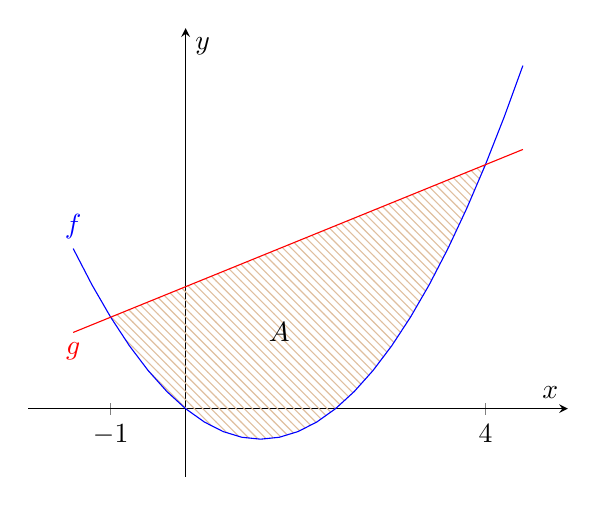
\begin{tikzpicture}
         \begin{axis}[axis lines=middle,
           xlabel=$x$,
           ylabel=$y$,
           enlargelimits,
           ytick=\empty,
           xtick={-1,4},
           xticklabels={$-1$,$4$}]
           \addplot[name path=F,blue,domain={-1.5:4.5}] {x^2-2*x}
           node[pos=0, above]{$f$};
           
           \addplot[name path=G,red,domain={-1.5:4.5}] {x+4}
           node[pos=0, below]{$g$};
           
           \addplot[pattern=north west lines, pattern color=brown!50]fill between[of=F and G, soft clip={domain=-1:4}]
           ;
           \path (1.25,2.5) node{$A$};
         \end{axis}
       \end{tikzpicture}
       &
         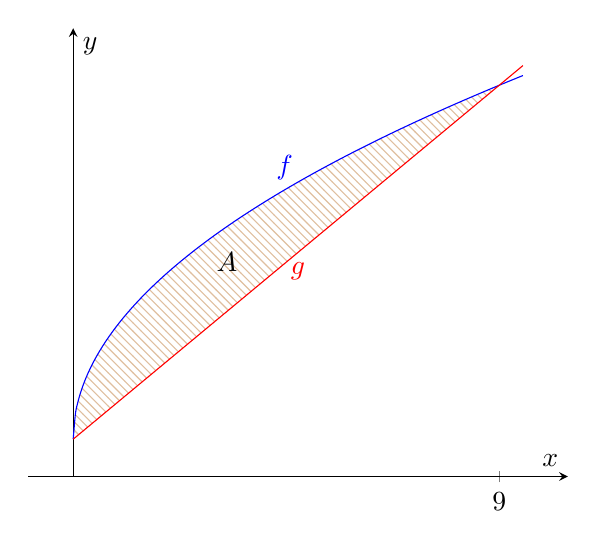
\begin{tikzpicture}
           \begin{axis}[axis lines=middle,
             samples=200,
             xlabel=$x$,
             ylabel=$y$,
             enlargelimits,
             ytick=\empty,
             xtick={0,9},
             xticklabels={$0$,$9$}]
             \addplot[name path=F,blue,domain={0:9.5},smooth] {1+sqrt(x)}
             node[pos=0.5, above]{$f$};
             
             \addplot[name path=G,red,domain={0:9.5}] {(3+x)/3}
             node[pos=0.5, below]{$g$};
             
             \addplot[pattern=north west lines, pattern color=brown!50]fill between[of=F and G, soft clip={domain=0:9}]
             ;
             \path (3.25,2.5) node{$A$};            
           \end{axis}
         \end{tikzpicture}
       \\
       \mbox{(a) $y=f(x) = x^2-2x$, $y=g(x)=x+4$}
       &
         \mbox{(b) $y=f(x)=1+\sqrt{x}$, $y=g(x)=(3+x)/3$}
       \\
       \\
       \\
       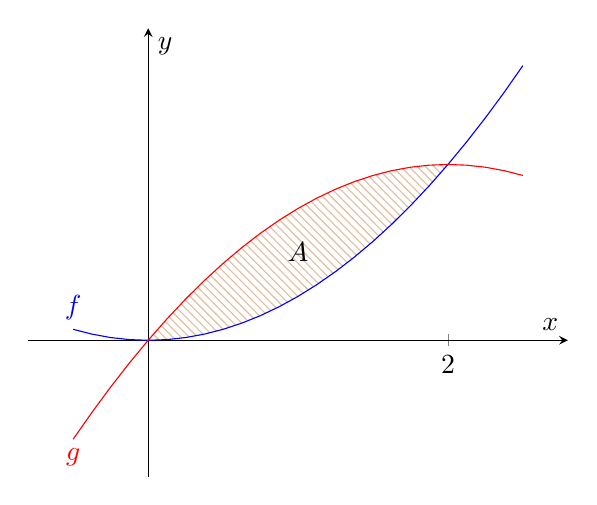
\begin{tikzpicture}
         \begin{axis}[axis lines=middle,
           xlabel=$x$,
           ylabel=$y$,
           enlargelimits,
           ytick=\empty,
           xtick={0,2},
           xticklabels={$0$,$2$}]
           \addplot[name path=F,blue,domain={-0.5:2.5}] {x^2}
           node[pos=0, above]{$f$};
           
           \addplot[name path=G,red,domain={-0.5:2.5}] {4*x-x^2}
           node[pos=0, below]{$g$};
           
           \addplot[pattern=north west lines, pattern color=brown!50]fill between[of=F and G, soft clip={domain=0:2}]
           ;
           % \node[coordinate,pin=60:{$A$}] at (axis cs:0.5,2.6){};
           \path (1,2) node {$A$};
         \end{axis}
       \end{tikzpicture}
       &
         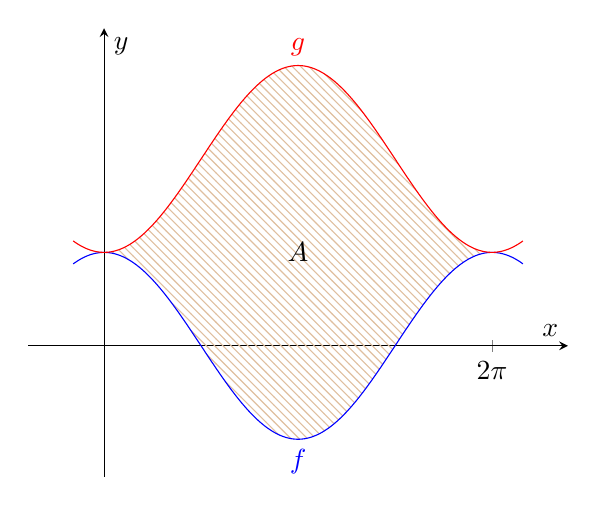
\begin{tikzpicture}
           \begin{axis}[axis lines=middle,
             samples=100,
             xlabel=$x$,
             ylabel=$y$,
             enlargelimits,
             ytick=\empty,
             xtick={0,6.283},
             xticklabels={$0$,$2\pi$}]
             \addplot[name path=F,blue,domain={-0.5:6.783},smooth] {cos(deg(x))}
             node[pos=0.5, below]{$f$};
             
             \addplot[name path=G,red,domain={-0.5:6.783},smooth] {2-cos(deg(x))}
             node[pos=0.5, above]{$g$};
             
             \addplot[pattern=north west lines, pattern color=brown!50]fill between[of=F and G, soft clip={domain=0:6.283}]
             ;
             % \node[coordinate,pin=60:{$A$}] at (axis cs:0.5,2.6){};
             \path (3.1415,1) node{$A$};
           \end{axis}
         \end{tikzpicture}
       \\
       \mbox{(c) $y=f(x)=x^2$, $y=g(x)=4x-x^2$}
       &
         \mbox{(d) $y=f(x)=\cos x$, $y=g(x)=2-\cos x$}
     \end{array}$
     \caption{Graphs for Question 1}
     \label{fig:ps051:1abcd}
  \end{figure}
\item These problems are harder than the previous, for various
  different reasons.  See Figure~\ref{fig:ps051:2abcd} on
  page~\pageref{fig:ps051:2abcd} for the graphs.
  \begin{enumerate}
  \item In this case, it's better to think of the curves as functions
    of $y$ instead of $x$.  For one thing, when we write
    $4x+y^2=12$ as a function of
    $y$, it is a polynomial, but if we write it at as a function of
    $x$, it uses a square root, which may be harder to integrate.  For
    another, $y^2 = 12-4x$ has two branches,
    $y=\sqrt{12-4x}$ and
    $y=-\sqrt{12-4x}$, both of which are involved in this question,
    complicating the analysis.  Note that $x=f(y) =
    3-y^2/4$ is greater than $x=g(y) =
    y$ in the region of interest.  The intersections are when
    \begin{equation*}
      3-y^2/4 = y \implies y^2 + 4y - 12 = 0 \implies (y+6)(y-2)=0
    \end{equation*}
    i.e., when $y=-6$ and $y=2$, so the area is
    \begin{equation*}
      \int_{-6}^2 (f(y)-g(y)) \; dy
      = \int_{-6}^2 \left(3 - \frac{y^2}{4} - y\right) \; dy
      = \left. \vphantom{\int} 3y - \frac{y^3}{12} - \frac{y^2}{2}
      \right|_{-6}^2
      = 6 - \frac{2}{3} - 2 + 18 - 18 + 18 = \frac{64}{3}
    \end{equation*}
  \item From the graph we see $y=f(x)=\sin(\pi x/2)$ is above
    $y=g(x)=x$ in the region of interest.  The curves intersect when
    \begin{equation*}
      \sin (\frac{\pi x}{2}) = x
    \end{equation*}
    which is an equation we don't know how to solve.  Instead, we try
    to guess the solutions.  When $x=0$, $\sin(\pi 0/2) = \sin 0 = 0$,
    so $x=0$ is a solution.  When $x=1$, $\sin(\pi 1/2) = \sin \pi/2 =
    1$, so $x=1$ another solution.  There is yet another solution when
    $x=-1$ (check it).  For now, let's just concentrate on the
    interval $[0,1]$.  We'll deal with $[-1,0]$ later.  We have
    \begin{equation*}
      A_1 = \int_0^1 (f(x)-g(x)) \; dx
      = \int_0^1 \left( \sin(\frac{\pi x}{2}) - x \right) \; dx
      = \left. \vphantom{\int} -\frac{2}{\pi} \cos(\frac{\pi x}{2}) -
        \frac{x^2}{2} \right|_0^1
      = 0 - \frac{1}{2} + \frac{2}{\pi} - 0
      = \frac{2}{\pi}-\frac{1}{2}
    \end{equation*}
    Now, by symmetry, we can conclude that $A_2=A_1$, so altogether
    the area between the two curves is
    \begin{equation*}
      2A_1 = 2\left(\frac{2}{\pi}-\frac{1}{2}\right) = \frac{4}{\pi} - 1
    \end{equation*}
  \item The two curves coincide when
    \begin{equation*}
      \cos x = 1 - \cos x \implies 2\cos x = 1 \implies \cos x =
      \frac{1}{2}
      \implies x = \frac{\pi}{3}
    \end{equation*}
    There are other solutions to the equation, but they are outside of
    the interval $[0,\pi]$.  The area is in two parts; for $A_1$,
    $y=f(x)$ is above $y=g(x)$ so the area is
    \begin{equation*}
      A_1 = \int_0^{\pi/3} (f(x)-g(x)) \; dx
      = \int_0^{\pi/3} (2\cos x - 1) \; dx
      = \left. \vphantom{\int} 2\sin x -x \right|_0^{\pi/3}
      = \sqrt{3} - \frac{\pi}{3}
    \end{equation*}
    On the other hand, for $A_2$, the area is
    \begin{equation*}
      A_2 = \int_{\pi/3}^\pi (g(x)-f(x)) \; dx
      = \int_{\pi/3}^\pi (1-2\cos x) \; dx
      = \left. \vphantom{\int} x - 2\sin x \right|_{\pi/3}^\pi
      = \pi - \frac{\pi}{3} + \sqrt{3}
      = \frac{2\pi}{3} + \sqrt{3}
    \end{equation*}
    Altogether the area between the two curves in the domain $[0,\pi]$
    is
    \begin{equation*}
      A = A_1 + A_2 = \sqrt{3} - \frac{\pi}{3} + \frac{2\pi}{3} +
      \sqrt{3}
      = 2\sqrt{3} + \frac{\pi}{3}
    \end{equation*}
  \item We should write the absolute value function $|x|$ in terms of
    cases:
    \begin{equation*}
      |x| = \begin{cases} -x & \mbox{if $x\le 0$} \\ x & \mbox{if
          $x\ge 0$} \end{cases}
    \end{equation*}
    Next we find the intersections between $y=f(x)=|x|$ and
    $y=g(x)=x^2-2$ by solving two equations.  First, when $x\le 0$,
    $f(x)=-x$ so we have
    \begin{equation*}
      -x = x^2 - 2 \implies x^2 + x - 2 = 0 \implies (x+2)(x-1) = 0
    \end{equation*}
    We keep the solution $x=-2$ and drop the solution
    $x=1$ because it is outside the domain $x\le
    0$.  Similarly, when $x\ge 0$, $f(x)=x$ so we have
    \begin{equation*}
      x = x^2 - 2 \implies x^2 - x - 2 = 0 \implies (x+1)(x-2) = 0
    \end{equation*}
    We keep the solution $x=2$ and drop the solution $x=-1$ because it
    is outside the domain $x \ge 0$.  Now we are ready to find the
    area.  First we find the area
    \begin{equation*}
      A_1 = \int_{-2}^0 (f(x)-g(x)) \; dx
      = \int_{-2}^0 (-x - x^2 + 2) \; dx
      = \left. \vphantom{\int} -\frac{x^3}{3} - \frac{x^2}{2} + 2x
      \right|_{-2}^0
      = -\frac{8}{3} + \frac{4}{2} - 2(-2) = \frac{10}{3}
    \end{equation*}
    By symmetry, $A_2=10/3$ also.  (Or you can evaluate the relevant
    integral.)  Altogether, the area between the curves is
    \begin{equation*}
      A = A_1 + A_2 = \frac{20}{3}
    \end{equation*}
  \end{enumerate}
  \begin{figure}[p]
    \centering
    $\begin{array}{c@{\hspace{0.25in}}c@{\hspace{0.25in}}c}
       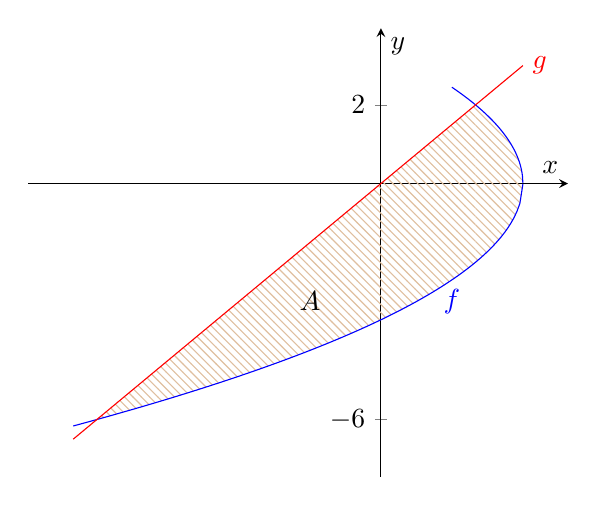
\begin{tikzpicture}
          \begin{axis}[axis lines=middle,
            samples=150,
            xlabel=$x$,
            ylabel=$y$,
            enlargelimits,
            ytick={-6,2},
            yticklabels={$-6$,$2$},
            xtick=\empty]
            %xticklabels={$-6$,$2$}]
            \addplot[name path=F,blue,domain={1.5:3}] {sqrt(12-4*x)};
            
            \addplot[name path=H,blue,domain={-6.5:3}] {-sqrt(12-4*x)}
            node[pos=0.75, below]{$f$};
            
            \addplot[name path=G,red,domain={-6.5:3}] {x}
            node[pos=1, right]{$g$};
            
            \addplot[pattern=north west lines, pattern color=brown!50]fill between[of=H and G, soft clip={domain=-6:2}]
            ;
            \addplot[pattern=north west lines, pattern color=brown!50]fill between[of=F and H, soft clip={domain=2:3}];
            \path (-1.5,-3) node{$A$};
          \end{axis}
        \end{tikzpicture}
        &
          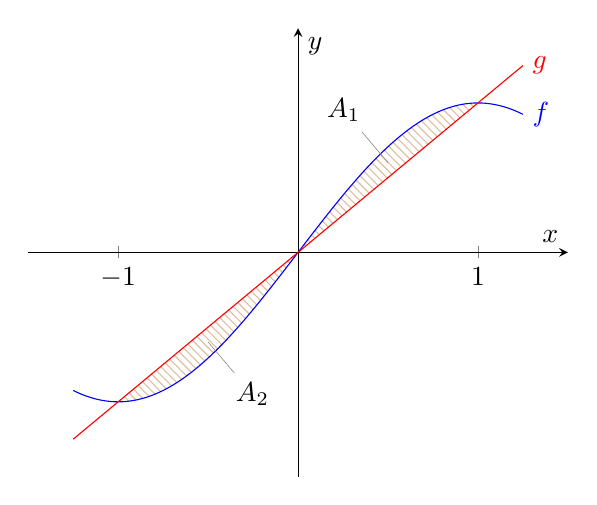
\begin{tikzpicture}
            \begin{axis}[axis lines=middle,
              samples=100,
              xlabel=$x$,
              ylabel=$y$,
              enlargelimits,
              ytick=\empty,
              xtick={-1,0,1},
              xticklabels={$-1$,$0$,$1$}]
              \addplot[name path=F,blue,domain={-1.25:1.25},smooth] {sin(deg((3.1415*x/2))}
              node[pos=1, right]{$f$};
              
              \addplot[name path=G,red,domain={-1.25:1.25}] {x}
              node[pos=1, right]{$g$};
              
              \addplot[pattern=north west lines, pattern color=brown!50]fill between[of=F and G, soft clip={domain=-1:1}]
              ;
              % \path (0.5,0.25) node{$A$};
              \node[coordinate,pin=300:{$A_2$}] at (axis cs:-0.5,-0.6){};
              \node[coordinate,pin=120:{$A_1$}] at (axis cs:0.5,0.6){};
            \end{axis}
          \end{tikzpicture}
        \\
        \mbox{(a) $4x+y^2=12$, $x=y$}
        &
          \mbox{(b) $y=\sin(\pi x/2)$, $y=x$}
        \\
        \\
        \\
        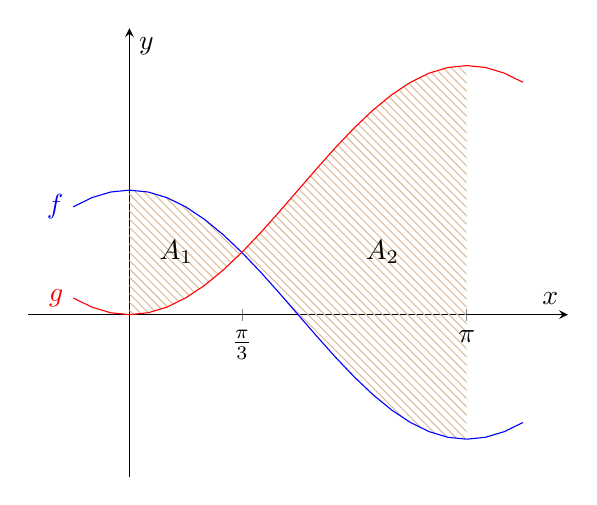
\begin{tikzpicture}
          \begin{axis}[axis lines=middle,
            xlabel=$x$,
            ylabel=$y$,
            enlargelimits,
            ytick=\empty,
            xtick={0,60,180},
            xticklabels={$0$,$\frac{\pi}{3}$,$\pi$}]
            \addplot[name path=F,blue,domain={-30:210}] {cos(x)}
            node[pos=0, left]{$f$};
            
            \addplot[name path=G,red,domain={-30:210}] {1-cos(x)}
            node[pos=0, left]{$g$};
            
            \addplot[pattern=north west lines, pattern color=brown!50]fill between[of=F and G, soft clip={domain=0:180}]
            ;
            % \node[coordinate,pin=60:{$A$}] at (axis cs:0.5,2.6){};
            \path (25,0.5) node{$A_1$};
            \path (135,0.5) node{$A_2$};
          \end{axis}
        \end{tikzpicture}
        &
          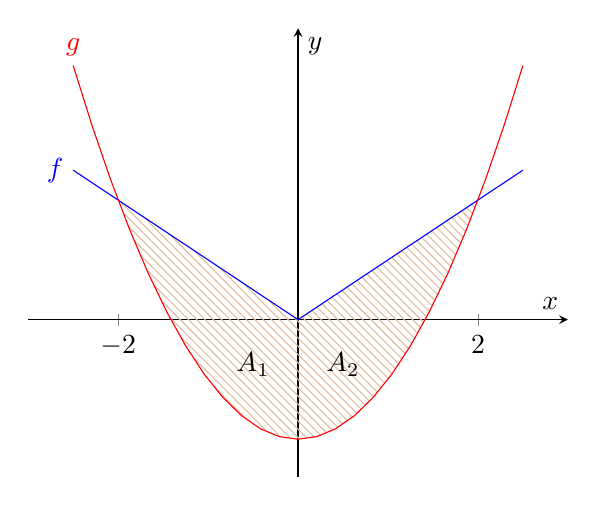
\begin{tikzpicture}
            \begin{axis}[axis lines=middle,
              xlabel=$x$,
              ylabel=$y$,
              enlargelimits,
              ytick=\empty,
              xtick={-2,2},
              xticklabels={$-2$,$2$}]
              \addplot[name path=F,blue,domain={-2.5:2.5}] {abs(x)}
              node[pos=0, left]{$f$};
              
              \addplot[name path=G,red,domain={-2.5:2.5}] {x^2-2}
              node[pos=0, above]{$g$};
              
              \addplot[pattern=north west lines, pattern color=brown!50]fill between[of=F and G, soft clip={domain=-2:2}]
              ;
              % \node[coordinate,pin=60:{$A$}] at (axis cs:0.5,2.6){};
              \path(-0.5,-0.75) node{$A_1$};
              \path(0.5,-0.75) node{$A_2$};
            \end{axis}
          \end{tikzpicture}
        \\
        \mbox{(c) $y=\cos x$, $y=1-\cos x$}
        &
          \mbox{(d) $y=|x|$, $y=x^2-2$}
    \end{array}$
    \caption{Graphs for Question 2}
    \label{fig:ps051:2abcd}
  \end{figure}
\item See Figure~\ref{fig:ps051:3} on page~\pageref{fig:ps051:3} for
    the graph.  The integral can be interpreted as the positive area
    between the two curves $y=f(x)=\sqrt{x+2}$ and $y=g(x)=x$.  We
    find the intersection points between the curves by solving
    \begin{equation*}
      \sqrt{x+2} = x \implies x+2 = x^2 \implies x^2 - x - 2 = 0
      \implies (x+1)(x-2) = 0
    \end{equation*}
    with solutions $x=2$, which we keep, and $x=-1$, which we discard
    because it is outside the domain $[0,4]$.  (It is also a
    ``spurious'' solution of the original equation.  If you substitute
    it back into the original equation, you'll find that it doesn't
    work.  Operations like squaring an equation may introduce such
    spurious solutions.)  The area can be found
    as the sum of two parts:
    \begin{equation*}
      A_1 = \int_0^2 (f(x)-g(x)) \; dx
      = \int_0^2 (\sqrt{x+2}-x) \; dx
      = \left. \vphantom{\int} \frac{2}{3} (x+2)^{3/2} - \frac{x^2}{2}
      \right|_0^2
      = \frac{16}{3} - 2 - \frac{2}{3} 2^{3/2}
      = \frac{10}{3} - \frac{4}{3} \sqrt{2}
    \end{equation*}
    and
    \begin{equation*}
      A_2 = \int_2^4 (g(x)-f(x)) \; dx
      = \int_2^4 (x-\sqrt{x+2}) \; dx
      = \left. \vphantom{\int} \frac{x^2}{2} - \frac{2}{3}(x+2)^{3/2}
      \right|_2^4
      = 8 - \frac{2}{3} 6^{3/2} - 2 + \frac{16}{3}
      = \frac{34}{3} - 4\sqrt{6}
    \end{equation*}
    Altogether the area between the curves is
    \begin{equation*}
      A = A_1 + A_2 = \frac{10}{3} - \frac{4}{3}\sqrt{2} +
      \frac{34}{3} - 4\sqrt{6}
      = \frac{44}{3} - \frac{4}{3}\sqrt{2} - 4\sqrt{6}
    \end{equation*}
  \begin{figure}[htbp]
    \centering
    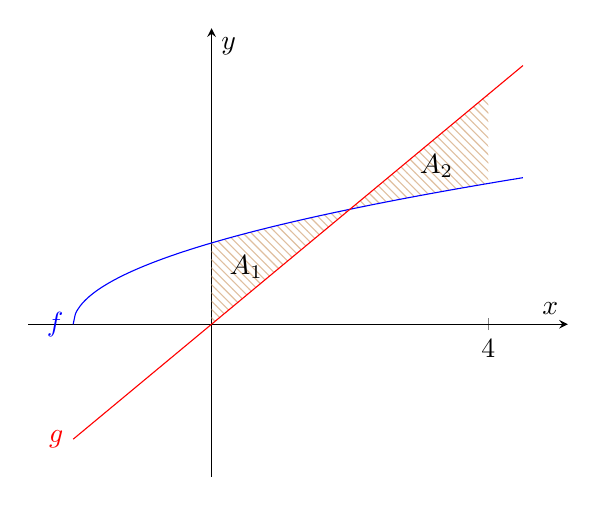
\begin{tikzpicture}
      \begin{axis}[axis lines=middle,
        samples=200,
        xlabel=$x$,
        ylabel=$y$,
        enlargelimits,
        ytick=\empty,
        xtick={0,4},
        xticklabels={$0$,$4$}]
        \addplot[name path=F,blue,domain={-2:4.5},smooth] {sqrt(x+2)}
        node[pos=0, left]{$f$};
        
        \addplot[name path=G,red,domain={-2:4.5}] {x}
        node[pos=0, left]{$g$};
        
        \addplot[pattern=north west lines, pattern color=brown!50]fill between[of=F and G, soft clip={domain=0:4}]
        ;
        \path (0.5,1) node{$A_1$};
        \path (3.25,2.75) node{$A_2$};            
      \end{axis}
    \end{tikzpicture}
    \caption{Graph for Question 3}
    \label{fig:ps051:3}
  \end{figure}
\item See Figure~\ref{fig:ps051:4} on page~\pageref{fig:ps051:4} for
  the graph.  The area of the region between the birth rate and death
  rate curves is the net change in population over the 10 year period,
  by the Net Change Theorem.  It is
  \begin{multline*}
    \int_0^{10} (2200+52.3t+0.74t^2-1460-28.8t) \; dt
    = \int_0^{10} (0.74 t^2 + 23.5 t + 740) \; dt
    = \left. \vphantom{\int} 0.247 t^3 + 11.75 t^2 + 740 t
    \right|_0^{10}
    \\
    = 247 + 1175 + 7400
    = 8822
  \end{multline*}
  \begin{figure}[htbp]
    \centering
    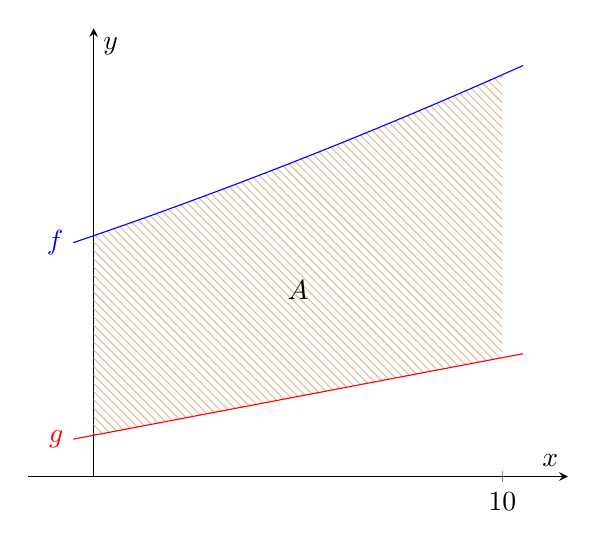
\begin{tikzpicture}
      \begin{axis}[axis lines=middle,
        xlabel=$x$,
        ylabel=$y$,
        enlargelimits,
        ytick=\empty,
        xtick={0,10},
        xticklabels={$0$,$10$}]
        \addplot[name path=F,blue,domain={-0.5:10.5},smooth] {2200+52.3*x+0.74*x^2}
        node[pos=0, left]{$f$};
        
        \addplot[name path=G,red,domain={-0.5:10.5}] {1460+28.8*x}
        node[pos=0, left]{$g$};
        
        \addplot[pattern=north west lines, pattern color=brown!50]fill between[of=F and G, soft clip={domain=0:10}]
        ;
        % \path (0.5,1) node{$A_1$};
        % \path (3.25,2.75) node{$A_2$};
        \path (5,2000) node{$A$};
      \end{axis}
    \end{tikzpicture}
    \caption{Graph for Question 4}
    \label{fig:ps051:4}
  \end{figure}
\item See Figure~\ref{fig:ps051:5} on page~\pageref{fig:ps051:5} for
  the graph.  First, we have to find the tangent line.  The slope of
  the tangent line is $(d/dx)\; x^2 = 2x$; the slope when $x=1$ is $m=2$.
  The point-slope equation for the tangent line is
  \begin{equation*}
    y - 1 = 2(x-1) \implies y-1 = 2x - 2 \implies y = 2x-1
  \end{equation*}
  The tangent line only intersects the curve when $x=1$ because
  \begin{equation*}
    2x-1 = x^2 \implies x^2 - 2x + 1 = 0 \implies (x-1)^2 = 0
  \end{equation*}
  which has only one solution, $x=1$.  Since the $x$-axis is also a
  boundary of the region in question, we need to find the intersection
  of the $x$-axis $y=0$ with the other two curves:
  \begin{equation*}
    x^2 = 0 \implies x=0
  \end{equation*}
  is the only intersection between the parabola and the $x$-axis, and
  \begin{equation*}
    2x-1 = 0 \implies x= \frac{1}{2}
  \end{equation*}
  is the only intersection between the $x$-axis and the tangent line.
  From the graph we can see that the area is
  \begin{equation*}
    \int_0^{1/2} (x^2 - 0) \; dx
    + \int_{1/2}^1 (x^2 - (2x-1)) \; dx
    = \left. \vphantom{\int} \frac{x^3}{3} \right|_0^{1/2}
    + \left. \vphantom{\int} \frac{x^3}{3} - x^2 + x \right|_{1/2}^1
    = \frac{1}{24} + \frac{1}{3} - 1 + 1 - \frac{1}{24} + \frac{1}{4}
    - \frac{1}{2}
    = \frac{1}{12}
  \end{equation*}
  \begin{figure}[htbp]
    \centering
    \begin{tikzpicture}
      \begin{axis}[axis lines=middle,
        xlabel=$x$,
        ylabel=$y$,
        enlargelimits,
        ytick=\empty,
        xtick={0,0.5,1},
        xticklabels={$0$,$\frac{1}{2}$,$1$}]
        \addplot[name path=F,blue,domain={0:1.25}] {x^2}
        node[pos=0, left]{$f$};
        
        \addplot[name path=G,red,domain={0:1.25}] {2*x-1}
        node[pos=0, left]{$g$};
        
        \addplot[name path=H,draw=none,domain={0:0.5}] {0};
        
        \addplot[pattern=north west lines, pattern color=brown!50]fill between[of=F and G, soft clip={domain=0.5:1}];
        
        \addplot[pattern=north west lines, pattern color=brown!50]fill between[of=F and H, soft clip={domain=0:0.5}];
        % \path (0.5,1) node{$A_1$};
        % \path (3.25,2.75) node{$A_2$};
        \node[coordinate,pin=100:{$A$}] at (axis cs:0.5,0.125){};
      \end{axis}
    \end{tikzpicture}
    \caption{Graph for Question 5}
    \label{fig:ps051:5}
  \end{figure}
\end{enumerate}
\end{document}
